\section{Illuminance calculation}
Illuminance $E$ of a planar surface is the areal density of luminous flux incident on the surface \cite{Habel}:

\begin{equation}
E=\frac{d\Phi_{i}}{dA}
\end{equation}

Where:
\begin{description}
	\item[$d\Phi_{i}$] is the luminous flux incident on a surface
	\item[$dA$] is the surface area
\end{description}

Luminous intensity $I$ is the amount of luminous flux contained in a given solid angle. For a direction defined by angle $\gamma$ is luminous intensity of this angle defined as follows \cite{Habel}:

\begin{equation}
I_{\gamma}=\frac{d\Phi}{d\Omega}
\end{equation}

Where:
\begin{description}
	\item[$d\Phi$] is the amount of luminous flux contained in the solid angle $d\Omega$
	\item[$d\Omega$] is the solid angle with its axis pointing in direction~$\gamma$
\end{description}

Illuminances mentioned in section~\ref{sec:Road_Lighting_Design} need to be calculated. Photometric properties of luminaires are defined in eulumdat files~\cite{Eulumdat}, containing luminous intensity distribution curves.

\begin{figure}[htb]
  \centering
  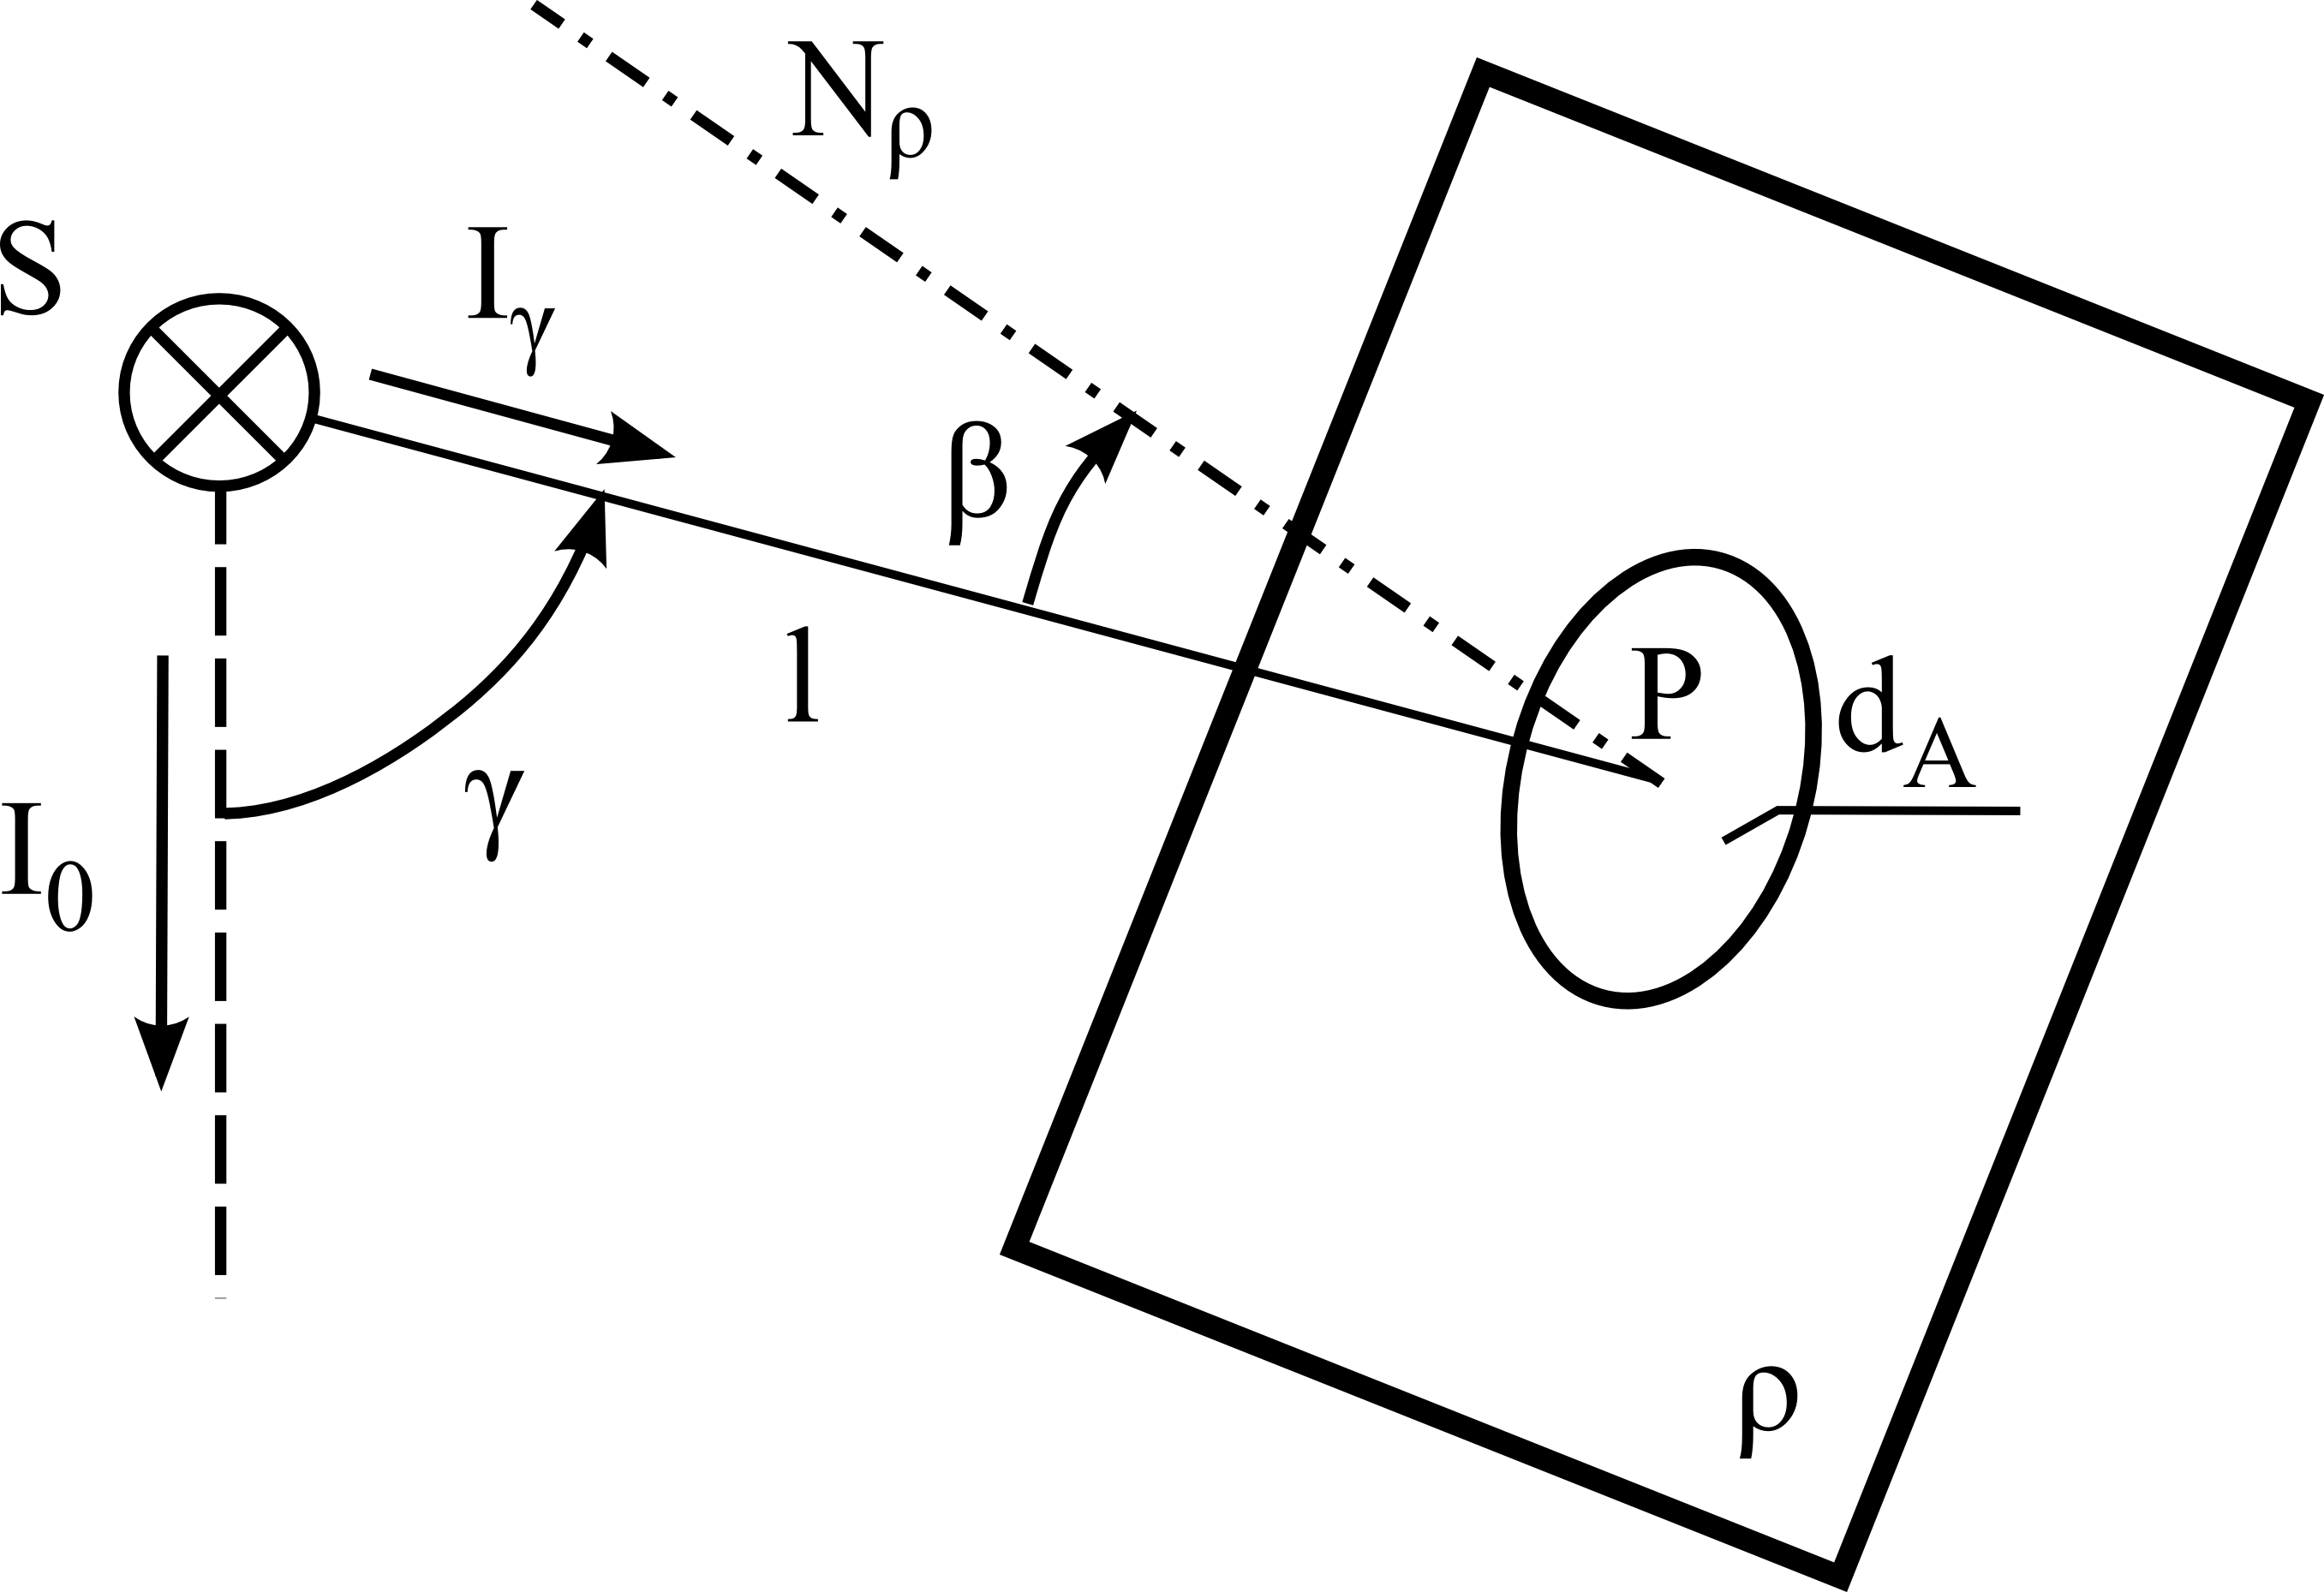
\includegraphics[width=0.8\columnwidth]{315_osvetlenost_bodovym_zdrojem}
  \caption{Facet $\rho$ illuminated with light source $S$}
  \label{fig:illuminance}
\end{figure}

According to~\cite{Habel} illuminance at point $P$ (as seen in figure~\ref{fig:illuminance}) illuminated by light source $S$ can be obtained by the following equation:

\begin{equation}
E_{P\rho}=\frac{I_{\gamma} \cdot cos \beta}{l^2}
\end{equation}

Where:
\begin{description}
	\item[$I_{\gamma}$] is the luminous intensity in the given direction $\gamma$
	\item[$\beta$] is the angle between the surface's normal $N_{\rho}$ and the $SP$ point join $l$
	\item[$l$] is the distance between the light source S and the point P of facet $dA$ of surface $\rho$
\end{description}

Luminous intensity distribution curves are presented in eulumdat files~\cite{Eulumdat} in the $C-\gamma$ coordinate system (figure~\ref{fig:Cgamma}). For photometric calculations in the situation of road lighting it is more suitable to use the $B-\beta$ coordinate system (figure~\ref{fig:Bbeta}), therefore it was necessary within the frame of this project to apply $B-\beta$ to $C-\gamma$ coordinate system conversion methods, allowing illuminance calculation algorithms to access the eulumdat file of the specific luminaire through the $B-\beta$ coordinate system.

\begin{figure}[htb]
  \centering
  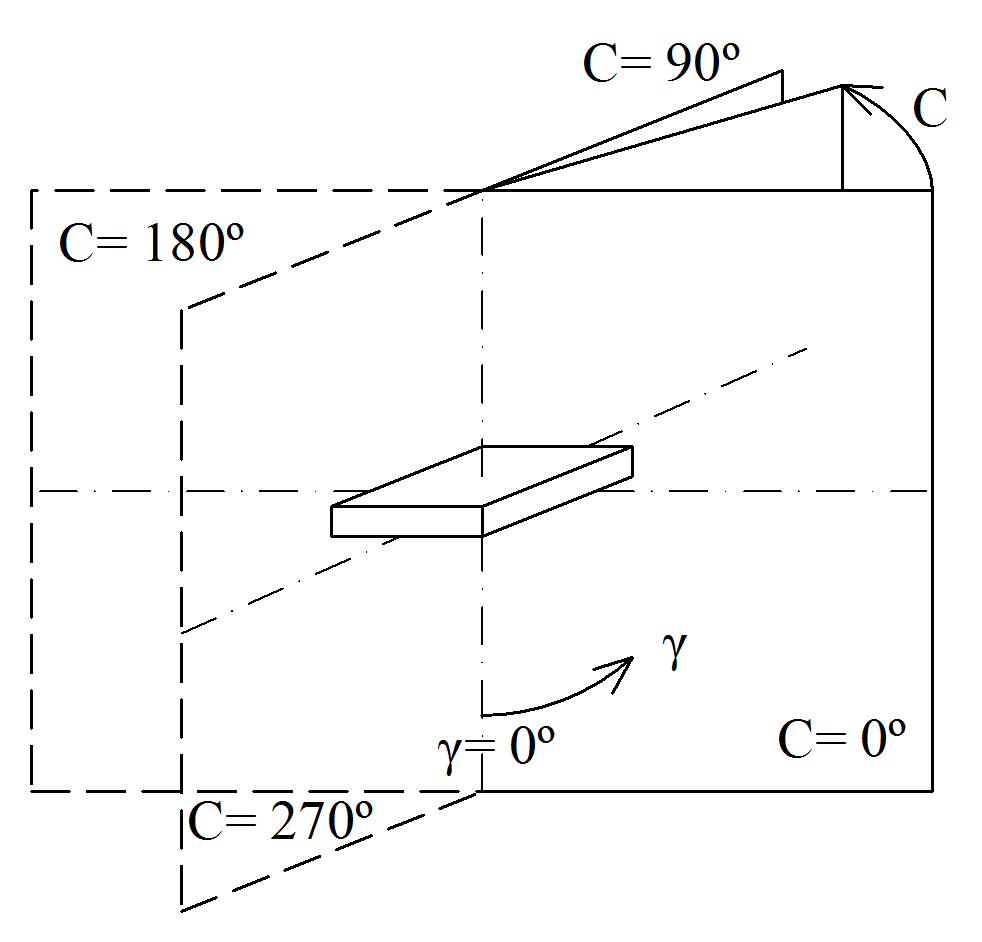
\includegraphics[width=0.65\columnwidth]{Cgama}
  \caption{$C-\gamma$ coordinate system}
  \label{fig:Cgamma}
\end{figure}

\begin{figure}[htb]
  \centering
  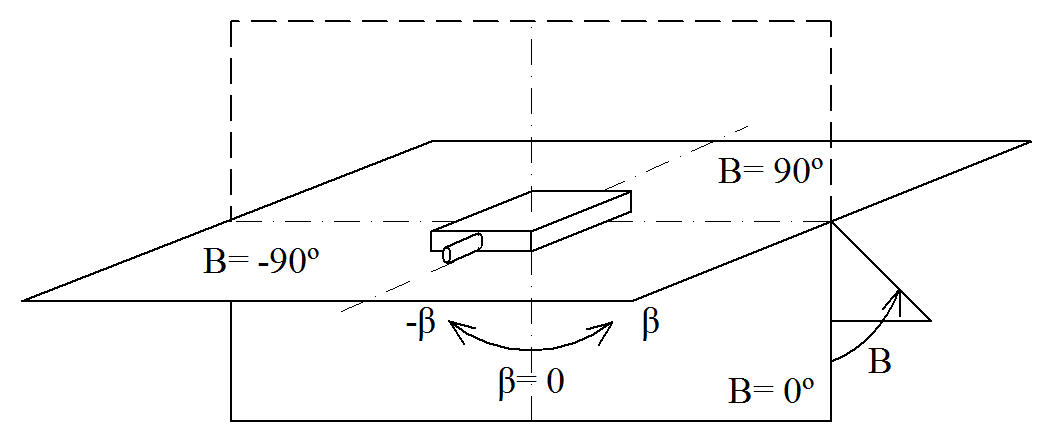
\includegraphics[width=\columnwidth]{Bbeta}
  \caption{$B-\beta$ coordinate system}
  \label{fig:Bbeta}
\end{figure}